\chapter{The Electronic Structure of Inorganic Benzenes: Valence Bond and Ring Current Descriptions}
\footnotetext{Reproduced with permission: ``The Electronic Structure of Inorganic Benzenes: Valence Bond and Ring Current Descriptions'', \mbox{J. J. Engelberts}, \mbox{R. W. A. Havenith}, \mbox{J. H. van Lenthe}, \mbox{L. W. Jenneskens} and \mbox{P. W. Fowler}, \textit{Inorg. Chem.} \textbf{2005}, \textit{44}, 5266-5272. \  \ \ \copyright 2005 American Chemical Society.}
\label{chap_inorganic}

\ifthenelse{\boolean{wholethesis}}{\relax}{\begin{center}\textit{Generated on \today\ at \currenttime}\end{center}}

\noindent\textbf{Abstract:}  Valence Bond (VB) theory and ring current maps have been used to study the electronic structure of inorganic benzene analogues X$_6$H$_6$ (X=C(\textbf{1}), Si (\textbf{2})),
X$_6$ (X=N(\textbf{3}), P(\textbf{4})), X$_3$Y$_3$H$_6$ (X,Y = B,N
(\textbf{5}), B,P (\textbf{6}), Al,N (\textbf{7}), Al,P (\textbf{8})) and
B$_3$Y$_3$H$_3$ (Y=O(\textbf{9}), S(\textbf{10})).
It is shown that the homonuclear compounds possess benzene-like character, with
resonance between two Kekul\'e-like structures, and induced diatropic
ring currents. Heteronuclear compounds typically show localization of the
lone-pairs on the electronegative atoms; Kekul\'e-like structures do not
contribute. Of the heteronuclear compounds, only B$_3$P$_3$H$_6$ (\textbf{6})
has some benzene-like features with a
significant contribution of two Kekul\'e-like structures to its VB wave
function, an appreciable resonance energy, and a discernible diatropic
ring current in planar geometry. However, relaxation of \textbf{6} to the optimal non-planar
chair conformation is accompanied by onset of localization of ring current.

\newpage

\section{Introduction}

\lettrine{\initial{B}}{}enzene is the archetypal example of a molecule that possesses remarkable
physical properties arising from its delocalized $\pi$ electrons.
Historically, chemists have searched for other molecules that resemble
benzene. Borazine (B$_3$N$_3$H$_6$ (\textbf{5})) and boroxine (B$_3$O$_3$H$_3$ (\textbf{9}))
are examples that have been proposed: in geometry and formal topology of the
$\pi$ molecular orbitals both are similar to benzene. However, the question of
whether their $\pi$ electrons are delocalized in the same sense as they are in
benzene (resonance between two Kekul\'e structures), is less clear. 

Aromaticity has many definitions.
Bond length equalization \cite{arom1}, extra energetic
stabilization \cite{arom2} with respect to an often hypothetical reference
system, and the ability to sustain an induced diatropic ring current \cite{ring4,ring1,ring2,ring3,nics}
have all been proposed as
descriptors for aromaticity. Many studies have been devoted to the aromaticity
of benzene analogues using concepts of aromatic stabilization energy (ASE),
exaltation of diamagnetizability $\Lambda$, and Nucleus Independent Chemical
Shift (NICS \cite{nics}) \cite{fink,jemmis,cooper,fowler1,schleyer1,soncini1}. On
these criteria, ``inorganic benzenes'' such as borazine (B$_3$N$_3$H$_6$ (\textbf{5})),
boroxine (B$_3$O$_3$H$_3$ (\textbf{9})) and borthiin (B$_3$S$_3$H$_3$ (\textbf{10})) are non-aromatic,
whereas $s$-triphosphatriborin (B$_3$P$_3$H$_6$ (\textbf{6})), hexaazabenzene (N$_6$ (\textbf{3})),
hexaphosphabenzene (P$_6$ (\textbf{4})), and hexasilabenzene (Si$_6$H$_6$ (\textbf{2})) are of modest
aromatic character \cite{schleyer1}.

An important question is whether the electronic structure of an inorganic
benzene expressed in terms of Lewis structures resembles that of benzene
itself. Valence Bond (VB) theory \cite{heitler}, where a molecular wave
function is constructed from atomic states, offers an interpretation precisely
in terms of resonating Lewis structures \cite{lewis}. Weights can be attributed
to these structures, using a formula proposed by Chirgwin and Coulson to assess
their importance in the total wave function \cite{chirgwin}. Furthermore, VB
provides a resonance energy ($E_{\mathrm{res}}$) of a molecule, as
defined by Pauling \cite{pauling}; this is the difference between the
total energy ($E_{\mathrm{tot}}$) and that of the most stable
structure. For benzene itself, a large value of 
$E_{\mathrm{res}}$=85--190 kJ/mol with respect to one
structure is found \cite{benzbovb,nature,fokke}. The structure with the lowest energy is
of the Kekul\'e type and has the largest weight in the wave function. Thus,
for benzene (\textbf{1}), aromaticity is characterized not only by a high
resonance energy, but also by large weights of the Kekul\'e
structures in the wave function.

In contrast, for the heteronuclear analogues borazine (\textbf{5}) and boroxine (\textbf{9}),
spin-coupled Valence Bond calculations indicate that only one Lewis structure,
corresponding to a description of three lone-pairs localized on the
electronegative centers, is important in the wave function, and
$E_{\mathrm{res}}$ is negligible \cite{cooper}. Significantly, the negligible
resonance energy coincides with the absence of a diatropic $\pi$ ring current, and so
energetic and magnetic criteria of aromaticity are in agreement here \cite{fowler1}.

The aim of the present chapter is to explore the parallels between the
energetic and magnetic criteria of aromaticity for a series of inorganic
benzenes, using VB methods for evaluation of resonance energy ($E_\mathrm{res}$), and
distributed origin computation of induced current density to establish
presence or absence of ring currents. VB calculations are performed using both
the strictly atomic model and the spin-coupled method. The magnetic response treatment is
carried out at the coupled Hartree-Fock
level \cite{ctocd-dz2,ctocd-dz3} using the ``ipsocentric''
 \cite{big,small} CTOCD-\textit{DZ} \cite{ctocd-dz4} approach, which is derived from the CSGT
method of Keith and Bader \cite{ctocd-dz1}, and which provides maps of induced
current density that give detailed information about the nature and
distribution of currents, and rationalize other magnetic indices of
aromaticity.

A set of candidate inorganic benzenes was defined (with benzene itself
included for comparison) as: X$_6$H$_6$ (X=C(\textbf{1}), Si (\textbf{2})),
X$_6$ (X=N(\textbf{3}), P(\textbf{4})), X$_3$Y$_3$H$_6$ (X,Y = B,N
(\textbf{5}), B,P (\textbf{6}), Al,N (\textbf{7}), Al,P (\textbf{8})) and
B$_3$Y$_3$H$_3$ (Y=O(\textbf{9}), S(\textbf{10})). Computed data on electric \cite{lazzeretti}
and magnetic \cite{schleyer1} properties of some of the molecules in the set are available
in the literature, including a
full set of NICS(0) \cite{nics} values for all molecules studied here.    

\section{Computational Details}

\subsection{Geometry Optimization}

Geometries of the molecules were optimized with GAMESS-UK  \cite{gamess} at the
DFT level, using the B3LYP functional (Table \ref{ch6.table1}) \cite{b3lyp1,b3lyp2,b3lyp3}.
\begin{table}[htdp]
\caption{Energetic and structural data for the set of candidate inorganic benzenes.}
\begin{center}
\begin{tabular}{c r r r c c}
\hline
\textbf{Compound}&
\textit{R}(\AA)${}^{a}$& 
$E_{\mathrm{tot,B3LYP}}$ ($E_{\mathrm{h}}$)${ }^{b}$&
$E_{\mathrm{tot,RHF}}$ ($E_{\mathrm{h}}$)${ }^{c}$ &
\mbox{n$_{\mathrm{imag}}$}${}^{d}$ &
$\tilde{\nu}$ (cm$^{-1}$)${}^{e}$\\
\hline
C$_6$H$_6$ ($D_\mathrm{6h}$) (\textbf{1})&1.394&--232.308558& --230.712903&0&-\\
Si$_6$H$_6$ ($D_\mathrm{6h}$) (\textbf{2})&2.216&--1740.627621&--1736.868797&1 ($b_{2g}$)&140$i$\\
N$_6$ ($D_\mathrm{6h}$) (\textbf{3})&1.319&--328.360861& --326.437481&2 ($e_{2u}$, $b_{2u}$)&272$i$,173$i$\\
P$_6$ ($D_\mathrm{6h}$) (\textbf{4})&2.133&--2048.236337&--2044.263216&1 ($e_{2u}$)&62$i$\\
P$_6$ ($D_\mathrm{2}$) (\textbf{4})&2.131&--2048.242943&--2044.268177&0&-\\
&2.125&&&&\\
B$_3$N$_3$H$_6$ ($D_\mathrm{3h}$) (\textbf{5})&1.431&--242.748573& --241.165102&0&-\\
B$_3$P$_3$H$_6$ ($D_\mathrm{3h}$) (\textbf{6})&1.838&--1102.337952&--1099.713109&1 ($a_2^{\prime\prime}$)&96$i$\\
B$_3$P$_3$H$_6$ ($C_\mathrm{3v}$) (\textbf{6})&1.855&--1102.338684&--1099.724589&0&-\\
Al$_3$N$_3$H$_6$ ($D_\mathrm{3h}$) (\textbf{7})&1.803&--895.509723& --892.779481&0&-\\
Al$_3$P$_3$H$_6$ ($D_\mathrm{3h}$) (\textbf{8})&2.266&--1755.187284&--1751.462147&2 ($e^{\prime\prime}$, $a_2^{\prime\prime}$)&166$i$,151$i$\\
Al$_3$P$_3$H$_6$ ($C_\mathrm{s}$) (\textbf{8})&2.296&--1755.201278&--1751.471417&0&-\\
&2.316&&&&\\
&2.314&&&&\\
B$_3$O$_3$H$_3$ ($D_\mathrm{3h}$) (\textbf{9})&1.377&--302.403016& --300.701018&0&-\\
B$_3$S$_3$H$_3$ ($D_\mathrm{3h}$) (\textbf{10})&1.809&--1271.176315&--1268.490842&0&-\\
\\
\end{tabular}
\\
\flushleft
\begin{tabbing}
${}^{a}$ \= Ring bond length.\\
${}^{b}$ \> B3LYP optimized within symmetry constraints (see text).\\
${}^{c}$ \> RHF/6-31G** energy calculated at the B3LYP/\textbf{basis1} optimized geometry. The \\
              \> $\sigma$ orbitals from this calculation are retained in the VB procedure.\\
${}^{d}$ \> Number of imaginary frequencies. The symmetries of the imaginary modes are indicated\\ 
                \> between parentheses.  \\
${}^e$ \> Corresponding wave numbers ($\tilde{\nu}$) for compounds \textbf{1}-\textbf{10}. See Supporting Information. \\
\end{tabbing}
\label{ch6.table1}
\end{center}
\end{table}
For hydrogen, boron, carbon and nitrogen the \mbox{6-311$^{++}$G**} basis \cite{bs6_light,bs311ss,bspp}
and for the aluminum, phosphorus, sulphur and silicon the
\mbox{6-311G**} \cite{bs6_heavy,bs311ss} basis was used. We refer to this
combination as \textbf{basis1}. Heteronuclear rings were constrained
to $D_{\mathrm{3h}}$ symmetry, and homonuclear rings to
$D_{\mathrm{6h}}$ symmetry. Hessian calculations show the planar
symmetric geometries of \textbf{1}, \textbf{5}, \textbf{7}, \textbf{9} and
\textbf{10} to correspond to genuine minima on the potential energy
surface at this level of theory. For \textbf{2}, \textbf{3}, \textbf{4},
\textbf{6} and \textbf{8}, one (or more) imaginary frequencies were found,
indicating that the constrained structures are transition states (or higher order
saddle points). These results are in agreement with earlier
data \cite{geo1,geo2,geo3,geo4,geo5}. The relaxation of Si$_6$H$_6$ (\textbf{2}) from $D_\mathrm{6h}$
to $D_\mathrm{3d}$ symmetry is accompanied with a change in NICS(0) value from \mbox{--13.1 into
--11.0} \cite{baldridge}, indicating that the aromatic character is retained.
N$_6$ (\textbf{3}) is not stable, and dissociates into three separate N$_2$ molecules \cite{geo3},
and Al$_3$P$_3$H$_6$ (\textbf{8}) in the $D_\mathrm{3h}$ geometry shows no
aromatic character, a feature which will not change for the optimal $C_\mathrm{s}$ symmetry conformation.
Therefore, only the $D_\mathrm{6h}$ conformation of \textbf{2} and \textbf{3} and the $D_\mathrm{3h}$ conformation
of \textbf{8} are studied here. The $e_{2u}$ symmetry  of the imaginary
frequency for $D_\mathrm{6h}$-P$_6$ (\textbf{4}) suggests an out-of-plane distortion to $D_\mathrm{2}$, and
both conformations are studied. For B$_3$P$_3$H$_6$ (\textbf{6}), both the $D_\mathrm{3h}$ and the
chair ($C_\mathrm{3v}$) conformation, which corresponds to the minimum on
the potential energy surface, are investigated.

\subsection{Valence Bond Calculations}

VB/6-31G** \cite{bs6_light,bs6_heavy,bs31light_a,bs31light_b,bs31heavyss}//B3LYP/\textbf{basis1}
calculations were performed with TURTLE \cite{turtle} as implemented in the GAMESS-UK
package \cite{gamess}. In all calculations, frozen $\sigma$ orbitals were taken from a preceding
RHF/6-31G** calculation, and the $\pi$ system was described by six atomic
$p$ orbitals. Two types of calculations were carried out, \textit{viz.} strictly atomic, and
spin-coupled. 

In the \textit{strictly atomic} model, the orbitals were optimized using Valence Bond
Self Consistent Field (\mbox{VBSCF}) \cite{vbscf1, vbscf2}, but were forced to
remain on their initial centers throughout the optimization. The advantage of
this model is its clear interpretability in terms of well-defined Lewis
structures. Since the X and Y atoms can contribute 0, 1 or 2 electrons to the $\pi$ system
in a general X$_3$Y$_3$H$_n$ cycle, the wave function was accordingly constructed from Lewis
structures representing, respectively, the two Kekul\'{e} terms (\textbf{I} and
\textbf{II}), three lone-pairs on X (\textbf{III}), and three lone-pairs on Y
(\textbf{IV}) (Figure \ref{ch6.figure1}).

\begin{figure}[htbp]
\center
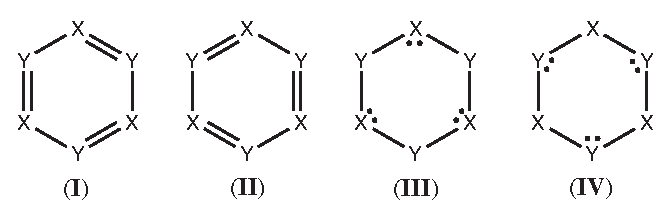
\includegraphics[scale=0.96]{inorganic/figures/figure1.eps}
\caption{The four structures used in strictly atomic VBSCF.}
\label{ch6.figure1}
\end{figure}

In order to partition the resonance energy ($E_\mathrm{res}$) into resonance interactions between
pairs of structures, the structures are orthogonalized using the criterion of
maximum overlap (L\"owdin orthogonalization \cite{lowdin}). The total energy
($E_\mathrm{tot}$) can then be divided into contributions from the
orthogonalized structures and their $\pi$ electron interactions
(resonances) \cite{remcolowdin}. The contribution of 
Kekul\'e-type resonance to the resonance energy ($E_\mathrm{res}$) can then be
expressed as a percentage of the total orthogonalized resonance energy.

The \textit{spin-coupled} Valence Bond wave function comprises one configuration
with all possible spin-couplings (two Kekul\'e and three Dewar structures) and
the orbitals are optimized without any restrictions \cite{scvb1,scvb2}.

\subsection{Calculation of the Induced Current Density}

Magnetic properties for all ten compounds were calculated with
SYSMO \cite{sysmo} at the coupled Hartree-Fock level within the
CTOCD-\textit{DZ}
formalism \cite{ctocd-dz2,ctocd-dz3,big,small,ctocd-dz1,ctocd-dz4}, and using
the \mbox{6-31G**} basis set \cite{bs6_light,bs6_heavy,bs31light_a,bs31light_b,bs31heavyss}
in the planar and planar-constrained geometries. Maps of $\sigma$, $\pi$ and total
($\sigma$+$\pi$) contributions to the current density were obtained. The
current density, induced by a unit magnetic field directed along the principal
axis, is plotted in a plane 1 $a_0$ above and parallel to the molecular plane.
Diatropic circulation is shown counterclockwise. As a quantitative indicator,
the maximum magnitude of the current density over each bond midpoint was
determined for $D_\mathrm{6h}$ \textbf{1}--\textbf{4}  in a square of dimension
2 $\times$ 2 $a_0$ centered on the point
midway between two neighboring atoms of the ring. 
For the maps of \textbf{4} and \textbf{6} in their non-planar, optimal structures, use was made of 
Pipek-Mezey \cite{pipek} localized orbitals in order to distinguish between the P--P single bonds
and the $\pi$ type orbitals.  The sum of the contributions of the three $\pi$ type orbitals
to the current density is plotted in various planes (see text) \cite{fowler2}.
Magnetic shielding values
at the ring center (--NICS(0) \cite{nics}) were obtained by
integration of the full 3D induced current density for the three directions of the external field,
using the CTOCD-\textit{PZ2} formalism \cite{ctocd-pz,soncini2}.

\section{Results}

\subsection{Valence Bond}

The results from the strictly atomic VBSCF calculations are reported in
Table \ref{ch6.table2}. For the X$_6$ ring compounds \textbf{1}--\textbf{4},
large weights for the Kekul\'e structures (W(\textbf{I}) and
W(\textbf{II})) and resonance energies $E_{\mathrm{res}}$ ranging
from 53.7 to 161.4 kJ/mol are found. 

\begin{table}[htdp]
\caption{The total energy ($E_\mathrm{tot}$) of the four structure strictly atomic VBSCF calculations,
the corresponding resonance energy ($E_\mathrm{res}$), and the contribution of the resonance between the orthogonalized Kekul\'e structures to the orthogonalized resonance energy (\%).
The last four columns contain the weights of the Kekul\'e structures (\textbf{I} and \textbf{II}) and
the lone-pair structures (\textbf{III} and \textbf{IV}) (Figure \ref{ch6.figure1}).}
\begin{center}
\begin{tabular}{ c r r r r r r r }
\hline
\textbf{Compound}&
$E_{\mathrm{tot}}$&
$E_{\mathrm{res}}$&
\%&
W(\textbf{I})&
W(\textbf{II})&
W(\textbf{III})&
W(\textbf{IV})\\
&($E_{\mathrm{h}}$)&(kJ/mol)&&&&&\\
\hline
C$_6$H$_6$ ($D_\mathrm{6h}$) (\textbf{1})&--230.632723&161.4&42&0.47&0.47&0.03&0.03\\
Si$_6$H$_6$ ($D_\mathrm{6h}$) (\textbf{2})&--1736.843163&71.3&46&0.48&0.48&0.02&0.02\\
N$_6$ ($D_\mathrm{6h}$) (\textbf{3})&--326.352653&138.8&59&0.49&0.49&0.01&0.01\\
P$_6$ ($D_\mathrm{6h}$) (\textbf{4})&--2044.248814&53.7&69&0.49&0.49&0.01&0.01\\
B$_3$N$_3$H$_6$ ($D_\mathrm{3h}$) (\textbf{5})&--241.032610&61.6&7&0.05&0.05&0.90&0.00\\
B$_3$P$_3$H$_6$ ($D_\mathrm{3h}$) (\textbf{6})&--1099.608270&132.6&17&0.21&0.21&0.58&0.00\\
Al$_3$N$_3$H$_6$ ($D_\mathrm{3h}$) (\textbf{7})&--892.689102&12.5&3&0.01&0.01&0.98&0.00\\
Al$_3$P$_3$H$_6$ ($D_\mathrm{3h}$) (\textbf{8})&--1751.396664&18.2&6&0.02&0.02&0.96&0.00\\
B$_3$O$_3$H$_3$ ($D_\mathrm{3h}$) (\textbf{9})&--300.569045&27.6&4&0.02&0.02&0.96&0.00\\
B$_3$S$_3$H$_3$ ($D_\mathrm{3h}$) (\textbf{10})&--1268.385041&34.3&7&0.04&0.04&0.92&0.00\\
\end{tabular}
\label{ch6.table2}
\end{center}
\end{table}

With the exception of B$_3$P$_3$H$_6$ (\textbf{6}) the heteronuclear ring compounds have a low
weight for the Kekul\'e structures. The lone-pair structure with two electrons
on each atom X (\textbf{III}) is dominant in the wave function (highest weight varying from 0.90 to 0.98).
$E_{\mathrm{res}}$ varies from 12.5 to 61.6 kJ/mol, except in \textbf{6}, for
which a substantially higher resonance energy of 132.6 kJ/mol is found. The contributions
to the resonance energy of the resonance between the orthogonalized
Kekul\'e structures are between 3 and 7\%, but 17\% for \textbf{6}.

In Table \ref{ch6.table3}, the results from the spin-coupled VB calculations
are presented. Whereas $E_{\mathrm{res}}$ is still appreciable for 
the homonuclear rings, it is close to zero for the heteronuclear rings \textbf{5},
and \textbf{7} -- \textbf{10}, but still significant for \textbf{6}.
All $E_\mathrm{res}$ values are lower than those obtained for the strictly atomic orbital model. 

\begin{table}[ht]
\caption{Total energy ($E_\mathrm{tot}$) and resonance energy ($E_\mathrm{res}$) from the spin-coupled orbital VBSCF calculations for \textbf{1}-\textbf{10}.}
\begin{center}
\begin{tabular}{ c r r }
\hline
\textbf{Compound}&
$E_{\mathrm{tot}}$&
$E_{\mathrm{res}}$\\
&($E_{\mathrm{h}}$)&(kJ/mol)\\
\hline
C$_6$H$_6$ ($D_\mathrm{6h}$) (\textbf{1})& --230.778804&81.4\\
Si$_6$H$_6$ ($D_\mathrm{6h}$) (\textbf{2})& --1736.915636&43.3\\
N$_6$ ($D_\mathrm{6h}$) (\textbf{3})& --326.543850&97.8\\
P$_6$ ($D_\mathrm{6h}$) (\textbf{4})& --2044.335507&47.1\\
B$_3$N$_3$H$_6$ ($D_\mathrm{3h}$) (\textbf{5})& --241.203143&0.7\\
B$_3$P$_3$H$_6$ ($D_\mathrm{3h}$) (\textbf{6})& --1099.736541&52.5\\
Al$_3$N$_3$H$_6$ ($D_\mathrm{3h}$) (\textbf{7})& --892.818391&0.0\\
Al$_3$P$_3$H$_6$ ($D_\mathrm{3h}$) (\textbf{8})&--1751.476886&0.2\\
B$_3$O$_3$H$_3$ ($D_\mathrm{3h}$) (\textbf{9})& --300.744566&0.1\\
B$_3$S$_3$H$_3$ ($D_\mathrm{3h}$) (\textbf{10})& --1268.507409&1.3\\
\end{tabular}
\label{ch6.table3}
\end{center}
\end{table}

Figure \ref{ch6.figure2} shows the two singly occupied $p$ orbitals of
\begin{figure}[htbp]
\center
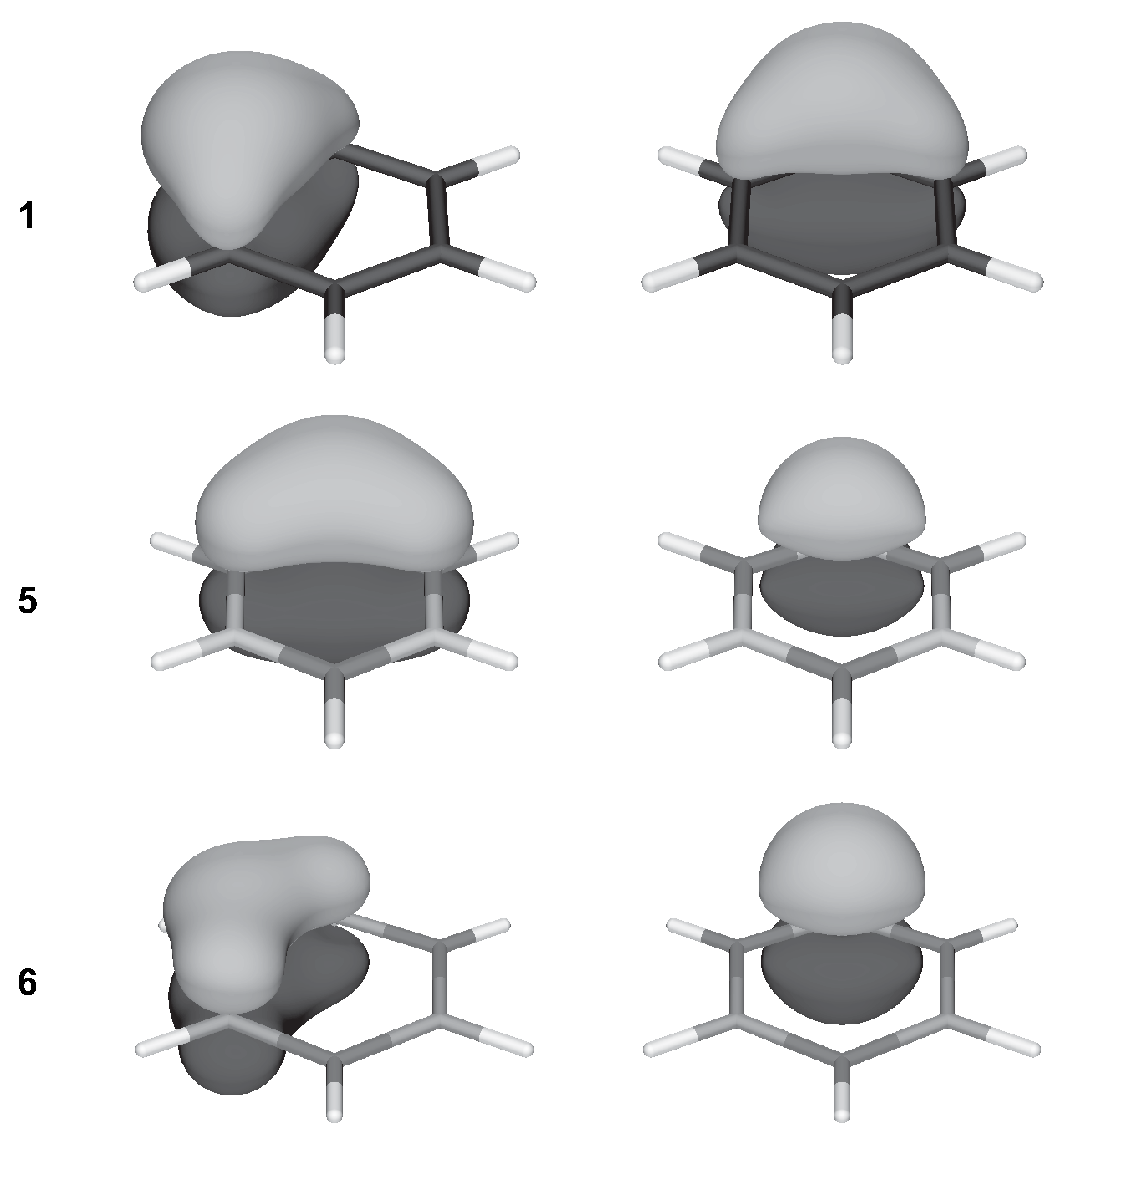
\includegraphics[scale=0.7]{inorganic/figures/figure2.eps}
\caption{A $p$ electron pair of C$_6$H$_6$ (\textbf{1}), B$_3$N$_3$H$_6$ (\textbf{5}) and B$_3$P$_3$H$_6$ (\textbf{6})
from top to bottom. Note that all spin-coupled calculations started with one $p$ orbital on each (hetero) atom.}
\label{ch6.figure2}
\end{figure}
benzene (\textbf{1}), borazine (\textbf{5}) and $s$-triphosphatriborin (\textbf{6}),
respectively. After the optimization of the spin-coupled wave function
\textbf{1} and \textbf{6} show
one $p$ orbital per atom with tails on both neighboring atoms, \textit{i.e.}
only a minor change from the starting position of a single $p$ orbital per
atom.  For \textbf{5} the orbital that originated from a boron atom migrates
completely to the nitrogen atom, leaving only small tails on the neighboring
boron atoms (\textit{cf.} Ref.  \cite{cooper}).

\subsection{Ring Currents}

From the plots of induced $\pi$ current density, computed in the ipsocentric approach, it can be deduced that the homonuclear rings support appreciable diatropic ring currents (Figure \ref{ch6.figure3}).
In contrast, the maps for the heteronuclear ring compounds show in all but one case, \textit{viz.} \textbf{6}, islands of localized currents centered around the electronegative atoms X. In the special case, \textbf{6}, there is a discernible diatropic $\pi$ ring current. The maps for \textbf{5} and \textbf{9} are similar to those previously reported \cite{fowler1,fowler2}.
\begin{figure}[htbp]
\center
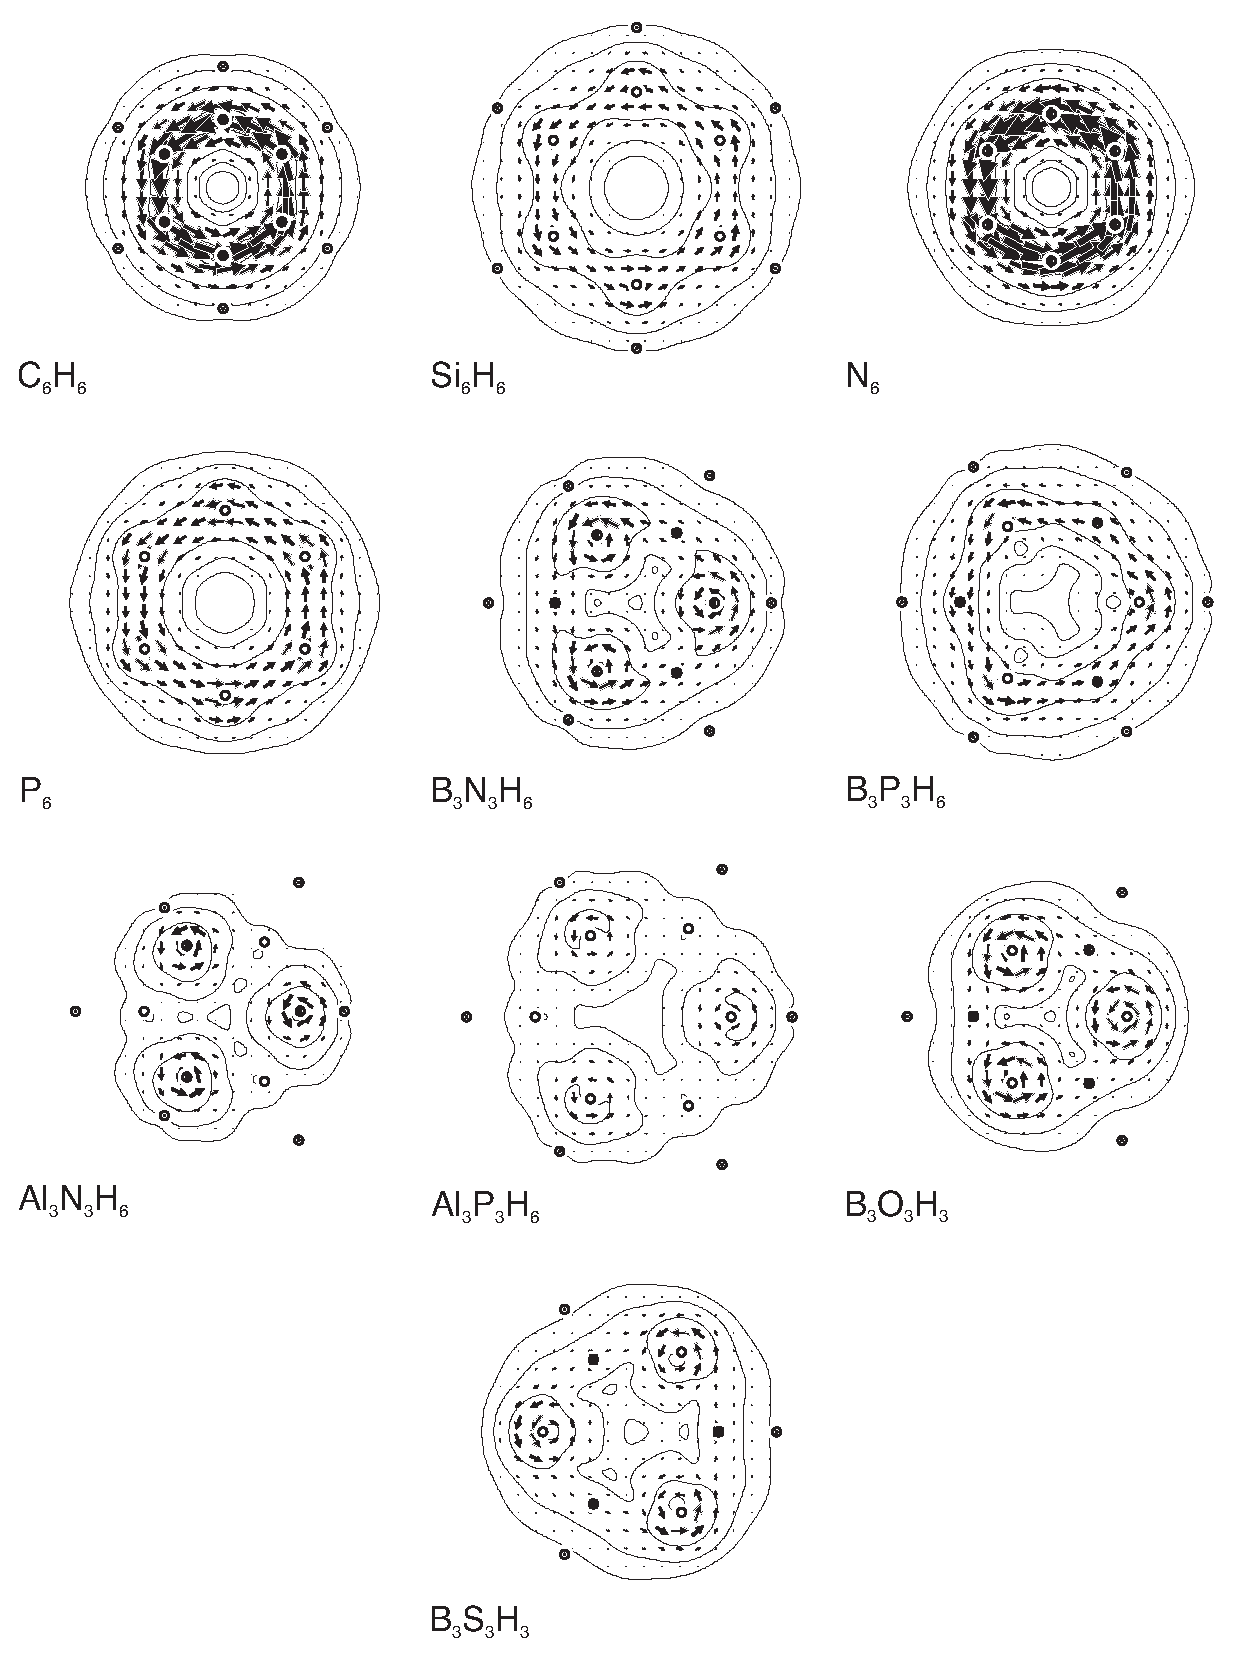
\includegraphics[scale=0.72]{inorganic/figures/figure3.eps}
\caption{Maps of $\pi$ current density induced by a perpendicular magnetic
field in planar geometries of compounds \textbf{1}-\textbf{10}. Current is plotted in
a plane 1 $a_{0}$ above the nuclei, with counterclockwise arrows indicating diatropic
circulation.}
\label{ch6.figure3}
\end{figure}
Sample $\sigma$ and total ($\sigma$+$\pi$) current-density maps for
\textbf{1}, \textbf{3}, \textbf{6} and \textbf{7} are shown in Figure \ref{ch6.figure4}.
Benzene (\textbf{1}) and N$_6$ (\textbf{3}) show the
profile familiar from many monocyclic and polycyclic compounds: superposition
of localized diatropic $\sigma$ bond currents leads to an outer diatropic
circulation and an inner paratropic central circulation within the ring.
\begin{figure}[htbp]
\center
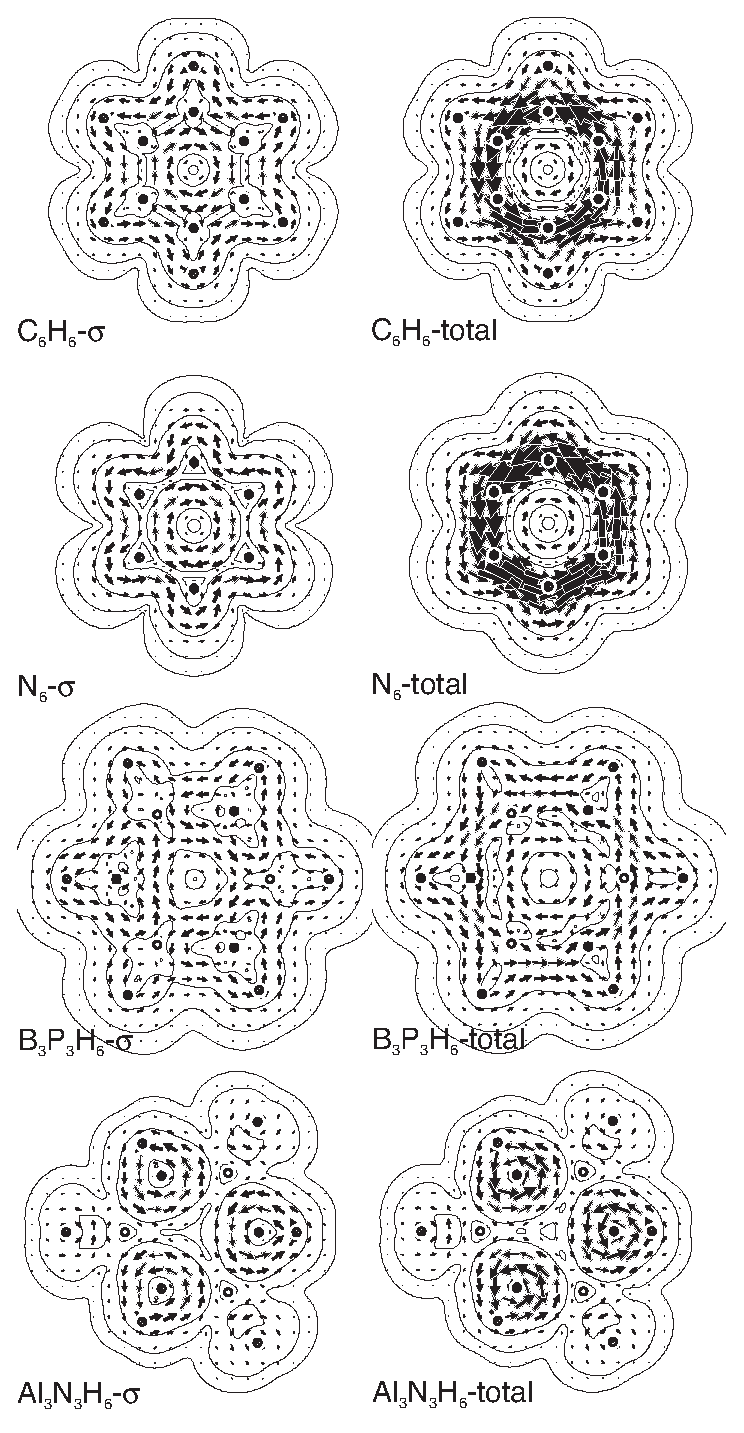
\includegraphics[scale=0.9]{inorganic/figures/figure4.eps}
\caption{Maps of the $\sigma$ (left) and the total ($\sigma$ + $\pi$) (right)
current density induced by a perpendicular magnetic field in planar geometries of
compounds \textbf{1}, \textbf{3}, \textbf{6} and \textbf{7} (from top to bottom). Current
is plotted in a plane 1 $a_{0}$ above the nuclei, with counterclockwise arrows
indicating diatropic circulation.}
\label{ch6.figure4}
\end{figure}
The localized compound Al$_3$N$_3$H$_6$ (\textbf{7}) shows a different $\sigma$ profile,
with three localized circulations around the electronegative centers
and no significant global perimeter circulation. In this context,
B$_3$P$_3$H$_6$ (\textbf{6}) appears again as a transitional system, with a
pattern that shows a tendency to localization of currents over the
electronegative phosphorus atoms, but with vestigial perimetric diatropic circulation.
Total ($\sigma$+$\pi$) maps at a height of 1 $a_{0}$ are dominated by the
$\pi$ ring currents in the homonuclear rings \textbf{1} and \textbf{3}, and by
the reinforcing lone-pair localized currents in \textbf{7}. Again,
B$_3$P$_3$H$_6$ (\textbf{6}) has a transitional character, with
counter-rotating perimetric and central currents, but without pronounced $\pi$
or $\sigma$ global ring current.
\begin{figure}[htbp]
\center
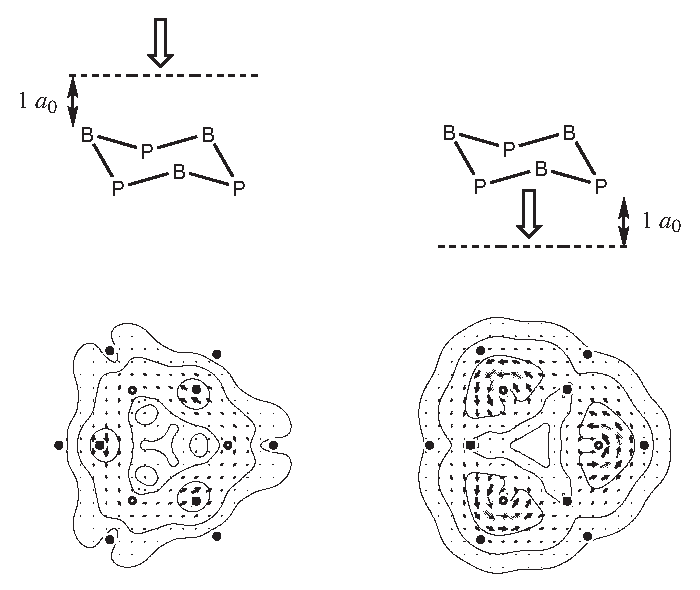
\includegraphics[scale=0.9]{inorganic/figures/figure5.eps}
\caption{ Maps of the induced $\pi$ current density induced by a magnetic field
acting along the principal axis for B$_3$P$_3$H$_6$ (\textbf{6}) in optimal $C_\mathrm{3v}$ symmetry
plotted in an plane 1 $a_0$ above the plane of boron nuclei (left) and 1 $a_0$ below the plane
of phosphorus nuclei (right) the molecule. The pictures above the maps indicate the plotting plane
(dashed lines) and the open arrow the direction of view.}
\label{ch6.figure5}
\end{figure}
Figure \ref{ch6.figure5} shows what happens to
the $\pi$ ring current of B$_3$P$_3$H$_6$ (\textbf{6}) on relaxation to its optimal
structure. The contribution of the orbitals derived from the $\pi$ orbitals
of the planar structure change from a global circulation to a set of localized 
islands, corresponding to the axial lone-pairs of the phosphorus atoms.
Shieldings at the ring center (\textit{cf.} --NICS(0) values) and the maximum magnitudes of 
$\pi$ current density ($j_{max}$) for the homonuclear rings are reported in
Table \ref{ch6.table4}. Broad agreement in size and sign is seen between
CTOCD-\textit{PZ2} mean shieldings and those previously
reported \cite{schleyer1}, in spite of differences in basis set, treatment of gauge and level
of electronic structure theory. An exception is the planar transition
state structure of P$_6$ (\textbf{4}), which shows, amongst others, a pronounced dependence on basis
set \cite{footnote,sadlej}. When
discussing $\pi$ ring currents, perhaps more significant than the value of the
average shielding is the out-of-plane component of the shielding
tensor, $\sigma_{zz}$, as this component reflects the effect of a
perpendicular magnetic field \cite{steiner2,corminboeuf,viglione}. The $\sigma_{zz}$
is calculated to be positive for all the homonuclear rings in the
set but negative for the heteronuclear compounds. Interestingly, B$_3$P$_3$H$_6$ (\textbf{6})
shows a near-zero computed value of $\sigma_{zz}$, (\textit{vide infra}).

\begin{table}[ht]
\caption{CTOCD-\textit{PZ2} components of the magnetic shieldings ($\sigma$) calculated at the ring center, the isotropic average ($\sigma_{av}$), literature NICS(0) values and the maximum modulus of the current density ($j_{max}$) for the studied compounds (\textbf{1}-\textbf{10}).}
\begin{center}
\begin{tabular}{ c rrr rr }
\hline
\textbf{Compound} &$-\sigma_{ip}^a$ & $-\sigma_{zz}$ & $-\sigma_{av}$ & NICS(0)$^b$ & $j_{max}$\\
\hline
C$_6$H$_6$ ($D_\mathrm{6h}$) (\textbf{1})& --11.0 & --16.4 & --12.8 &   --8.9 & 0.078\\
Si$_6$H$_6$ ($D_\mathrm{6h}$) (\textbf{2})& --10.9 & --16.7 & --12.8 &  --13.1 & 0.022\\
N$_6$ ($D_\mathrm{6h}$) (\textbf{3})& 1.8 &  --1.1 &   0.9 &   0.2 & 0.089\\
P$_6$ ($D_\mathrm{6h}$) (\textbf{4})& 6.9 & --14.2 &  --0.1 & --15.2 & 0.031\\
P$_6$ ($D_\mathrm{2}$) (\textbf{4})& 7.5 & --22.7 & --2.6 & - & - \\
B$_3$N$_3$H$_6$ ($D_\mathrm{3h}$) (\textbf{5})& --9.7 &  13.4 &  --2.0 &   --2.1 & -\\
B$_3$P$_3$H$_6$ ($D_\mathrm{3h}$) (\textbf{6})& --12.9 &   1.1 &  --8.2 &  --8.7 & -\\
B$_3$P$_3$H$_6$ ($C_\mathrm{3v}$) (\textbf{6})& --13.9 &   5.5 &  --7.4 &  - & -\\
Al$_3$N$_3$H$_6$ ($D_\mathrm{3h}$) (\textbf{7})& --8.9 &  11.1 &  --2.2 &   --2.4 & -\\
Al$_3$P$_3$H$_6$ ($D_\mathrm{3h}$) (\textbf{8})& --11.7 &   4.6 &  --6.3 &  --5.8 & -\\
B$_3$O$_3$H$_3$ ($D_\mathrm{3h}$) (\textbf{9})&  --8.0 &  20.0 &   1.4 &  --0.8 & -\\
B$_3$S$_3$H$_3$ ($D_\mathrm{3h}$) (\textbf{10})& --13.2 &  11.4 &  --5.0 &  --2.5 & -\\
\\
\end{tabular}
\\
\flushleft
$^a$ In-plane average $\sigma_{ip}=\frac{1}{2}(\sigma_{xx}+\sigma_{yy})$\\
$^b$ Taken from Ref.  \cite{schleyer1}\\
\label{ch6.table4}
\end{center}
\end{table}

\section{Discussion}

\subsection{Homonuclear X$_6$H$_n$ Series}

The four homonuclear compounds show ``aromatic'' behavior on both electronic
structure and magnetic indicators. A survey of the strictly atomic model results shows
that \textbf{1}--\textbf{4} have large Kekul\'e resonance contributions above
40\%, and high Kekul\'e structure weights (W(\textbf{I})=W(\textbf{II})), though explicit addition
of Lewis structures \textbf{III} and \textbf{IV} increases the resonance energy,
as it must by the variation principle. In the case of benzene, the inclusion of
\textbf{III} and \textbf{IV}, which gives an improvement of the wave function that is outside the
classical Kekul\'e resonance picture, amounts to an increase of about 52~kJ/mol.
All four molecules also display diatropic $\pi$ ring currents, as expected for aromatic
compounds, and there is qualitative correlation between the strength of current ($j_{max}$)
and the size of the resonance energy (Table \ref{ch6.table2}). C$_6$H$_6$ (\textbf{1}) and
planar N$_6$ (\textbf{3}) show strong ring currents and resonance energies ($E_\mathrm{res}$)
of 161.4 and 138.8~kJ/mol; planar Si$_6$H$_6$ (\textbf{2}) and P$_6$ (\textbf{4}) show ring currents
of less than half the benzene strength, and resonance energies ($E_\mathrm{res}$) of
 71.3 and 53.7~kJ/mol. The spin-coupled model shows lower resonance energies ($E_\mathrm{res}$)
than the strictly atomic method. In spin-coupled VB the orbitals have the freedom to spread out,
which means the implicit inclusion of ionic bond character. The only way to include ionic
character in the strictly atomic model is to mix the lone-pair structures \textbf{III}
and \textbf{IV} into the Kekul\'e picture of the homonuclear compounds and to mix the
Kekul\'e-type structures \textbf{I} and \textbf{II} into the lone-pair description of the
heteronuclear compounds. $E_\mathrm{res}$ is defined as the difference between the energy of the most stable structure and the total energy ($E_\mathrm{tot}$). The most stable spin-coupled structure
has a lower energy than the most stable structure in the strictly atomic model, leading to
a higher $E_\mathrm{res}$ for the strictly atomic model.

Interestingly, the magnetic aromaticity of the N$_6$ (\textbf{3}) ring is not captured by
calculating the NICS(0) index. As has been discussed elsewhere \cite{steiner1},
the isotropic central shielding that defines NICS is influenced by many factors in addition to
the $\pi$ ring currents; even restriction to the out-of-plane component of
shielding does not help here, as localized $\sigma$ and delocalized $\pi$ circulations give near canceling
contributions to $\sigma_{zz}$. Inspection
of the current-density map is more informative than either of these global
integral properties.

The ring current calculations on P$_6$ (\textbf{4}) require a more detailed explanation:
although $-\sigma_{av}$ is only --0.1 for planar \textbf{4}, the $\pi$ map
in Figure \ref{ch6.figure3} shows a strong ring current, and, consistent with this observation, the
$-\sigma_{zz}$-component is --14.2, indicating aromatic character. For the method and basis set
used here, the paratropic in-plane component of NICS exactly counteracts the diatropic
ring current component, whereas an enlargement of basis set leads to a similar $-\sigma_{zz}$,
but different in-plane average ($-\sigma_{ip}$) value (see also note  \cite{footnote}).

The deformation to the P$_6$ (\textbf{4}) optimal $D_2$ symmetric geometry does not quench the $\pi$ ring current, as shown in Figure \ref{ch6.figure6}.
\begin{figure}[htbp]
\center
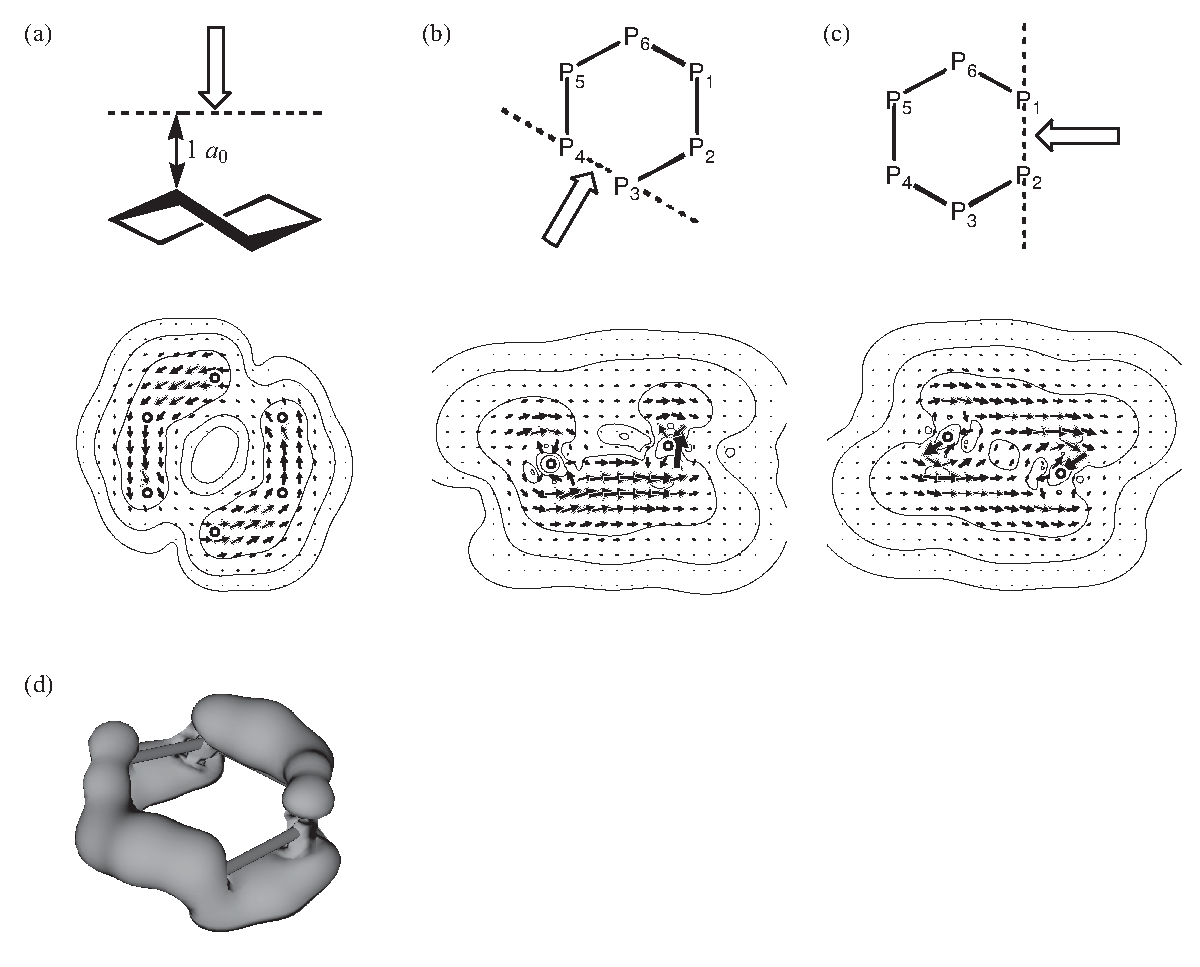
\includegraphics[scale=0.68]{inorganic/figures/figure6.eps}
\caption{Maps of the induced $\pi$ current density induced by a magnetic field acting perpendicular to
the median plane for P$_6$ (\textbf{4}) in optimal $D_2$ symmetry plotted in a plane (a) 1 $a_0$ above the top
two phosphorus nuclei, (b) containing the P$_3$--P$_4$ bond and the magnetic field, and (c) containing the
P$_1$--P$_2$ bond and the magnetic field; (d) contour plot of modulus of $\pi$ current-density (contour value: 0.024). 
Diatropic current is denoted by arrows pointing counterclockwise (a) and from left to right (b) and (c). 
The pictures above the maps indicate the plotting plane (dashed lines) and the open arrow the direction of view.}
\label{ch6.figure6}
\end{figure}
The side view plots through the
two symmetry unique \mbox{P$_1$--P$_2$} and \mbox{P$_3$--P$_4$} bonds show that the main
current along the \mbox{P$_3$--P$_4$} bond is concentrated on one side of the bond, while
along the \mbox{P$_1$--P$_2$} bond it is more evenly distributed.  A contour plot of the
modulus of $\pi$ current density (contour value 0.024) gives an indication of the current-path
in three dimensions (as do the arrows sometimes added to the plots of current-density anisotropy in the
ACID method \cite{herges}). This picture combined with
the side view plots show the continuous $\pi$ ring current and rationalize the gaps seen in
the map plotted 1.6 $a_{\mathrm{0}}$ above and parallel to the median plane.

\subsection{Heteronuclear X$_3$Y$_3$H$_n$ Series}

Our calculations give little support to any putative assignment of these
compounds as being ``aromatic''. All but B$_3$P$_3$H$_6$ (\textbf{6}) fit into a
simple pattern: they have low resonance energies ($E_{\mathrm{res}}$), large
weights for a localized lone-pair structure with low fractional contributions
of Kekul\'e resonances to $E_\mathrm{res}$. Maps of induced current density
show concomitant localization of the magnetic response.

Borazine (\textbf{5}) appears to be an exception to this pattern. In the strictly
atomic VB calculations, it shows a significant $E_\mathrm{res}$ value of 61.6 kJ/mol. Upon relaxation of
the constraint on the nature of the $p$ orbitals,
however, this $E_\mathrm{res}$ value is seen to have been an artifact. The improved $E_\mathrm{res}$ value, available from
the spin-coupled VB calculation, is negligible (0.7 kJ/mol). The maps
(Figure \ref{ch6.figure3}) do not show any evidence of benzenoid behavior.

In contrast, B$_3$P$_3$H$_6$ (\textbf{6}) possesses a large resonance
energy both in the strictly atomic and spin-coupled VBSCF calculations,
but its $-\sigma_{zz}$ value is 1.1. As shown in the maps in Figures \ref{ch6.figure3}
and \ref{ch6.figure4}, in the case of \textbf{6}, the weak diatropic $\pi$ current
is cancelled by paratropic contributions (see also N$_6$ (\textbf{3})), due to localized
$\sigma$ currents.  The average in-plane component of NICS(0), notwithstanding, is negative
($-\sigma_{ip}=-12.9$) leading to an aromatic overall $-\sigma_{av}$ (NICS(0)) of --8.2.  Hence,
for \textbf{6} total NICS(0) does not reflect the presence of an underlying ring current. An interesting critique of the NICS
approach in general is given in Ref.  \cite{paolo}.

The exceptional character of B$_3$P$_3$H$_6$ (\textbf{6}) is also reflected by the contour plots
of its spin-coupled orbitals in comparison with those of benzene (\textbf{1}) and borazine
(\textbf{5}) (Figure \ref{ch6.figure2}).  While for benzene (\textbf{1}), one singly occupied orbital on
each carbon atom is found, which can be interpreted as a covalent bond, for borazine
(\textbf{5}) two singly occupied orbitals centered on nitrogen are discernible, which
correspond to the description of a  nitrogen lone-pair.  B$_3$P$_3$H$_6$ (\textbf{6}) 
is formally more similar to borazine (\textbf{5}) but its orbitals are intermediate between
those of benzene (\textbf{1}) and borazine (\textbf{5}): one orbital is strictly centered
on phosphorus (similar to \textbf{5}), while the other orbital is centered on boron
(more benzenoid) with tails on phosphorus, representing the larger Kekul\'e-type
structure contributions due to the small difference in electronegativity between boron and
phosphorus  \cite{elecpauling}.  Thus, this pictorial result, together with the $E_\mathrm{res}$ of 52.5~kJ/mol
and the large Kekul\'e resonance contribution to the orthogonalized resonance energy suggests
that planar B$_3$P$_3$H$_6$  (\textbf{6}) is benzene-like. 

The current density maps give an indication of aromatic behavior
in \textit{planar} B$_3$P$_3$H$_6$ (\textbf{6}) in that the $\pi$ current pattern is delocalized,
though not uniform in strength. When the geometry is allowed to relax to the local $C_{\mathrm{3v}}$
minimum, the current changes from a global circulation to a
set of localized islands, corresponding to the \textit{axial} lone-pairs of the phosphorus atoms
(Figure \ref{ch6.figure6}). Thus according to the magnetic criterion, \textbf{6} is non-aromatic.

\section{Conclusions}

Three complementary theoretical techniques were used to explore the putative
aromaticity of a set of inorganic benzenes. Each technique gives a visualization
of aromaticity: strictly atomic VB calculations through the balance of Kekul\'e and
lone-pair structures, spin-coupled calculations through resonance energy, and the CTOCD-\textit{DZ}
current-density maps through distinction between global ring current and local circulations.

The strictly atomic model gives a clear division of the molecules into a
benzene-like group and a group with lone-pairs on the most electronegative
atoms. This division corresponds to that derived from the maps of magnetic response. The spin-coupled
method, which gives an improved description of the
electronic structure through unrestricted orbital optimization, leads to the same partitioning of the
set. If the label ``inorganic benzene'' is to be applied to any of the compounds studied, it is apparently
appropriate only for the homonuclear ring compounds and the constrained N$_6$ (\textbf{3}), and with
reservations, for the planar geometry of B$_3$P$_3$H$_6$ (\textbf{6}).

\section*{Acknowledgement}

We would like to thank P. Miedema and N. Smeenk for their contributions to the VB calculations on B$_3$N$_3$H$_6$ (\textbf{5}).
R.W.A.H. acknowledges financial support from the Netherlands Organization for Scientific Research (NWO), grant 700.53.401.
\\
\\
\noindent \textbf{Supporting Information Available:} Cartesian coordinates for B3LYP/\textbf{basis1} (non)-constrained
compounds \textbf{1}--\textbf{10}. This material is available free of charge via the Internet at
http://pubs.acs.org.

\bibliography{inorganic}
\bibliographystyle{../main/achemso}
